\section{Objectives and handout requirements}

Following handout PDF pages 107--110, deck 01 tests the unsafe same-type cascade in Fig.26.1; deck 02 compares Figs.26.4/26.5 under equal 10 fF coupling and a strength sweep; deck 03 answers Q1 on speed. The three decks contain nine completed analyses without errors or failed measurements. The simulator reports suppressed encrypted-block warning details, which does not establish a warning-free model.

\section{Circuits, conditions, and interpretation}

The supplied model is evaluated at a declared teaching condition of 1.0 V and 25°C, not a certified voltage rating or reproduction of the original 2.5 V process. Unless stated otherwise, Wn/Wp/L = 0.6/1.8/0.25 µm and output load is 5 fF. The clock period is 10 ns with 20 ps edges. Declared low/high diagnostic thresholds are 0.2/0.8 V; these are not extracted receiver noise margins.

The N-only domino uses two four-transistor dynamic NAND gates with their second inputs tied high, each followed by a static inverter. The N-P chain directly alternates four N/P dynamic stages. Both implement noninverting logic with equal output loads. The N-domino core contains 12 transistors and the N-P core 16. This compares the handout topologies, not equal transistor counts or optimized logical effort.

Every public deck contains only a \texttt{MODEL\_SETUP\_REQUIRED} comment; local model setup is required before execution. Neither model content nor loading paths are distributed. Figures use actual printed data; per-case CSV and measurement JSON files are in \texttt{results/}.

\section{Step 1: unsafe cascading}

Input A rises during precharge. When the clock rises at 2.5 ns, X and Y are initially high, so X initially enables the second stage. Although the first stage later discharges X, lost charge at Y has no active restoration path during evaluation. Y is 0.655339 V at 7 ns, below the 0.8 V high diagnostic threshold. Here the result is substantial high-level degradation rather than a complete discharge to zero; that distinction is retained.

\begin{figure}[htbp]\centering
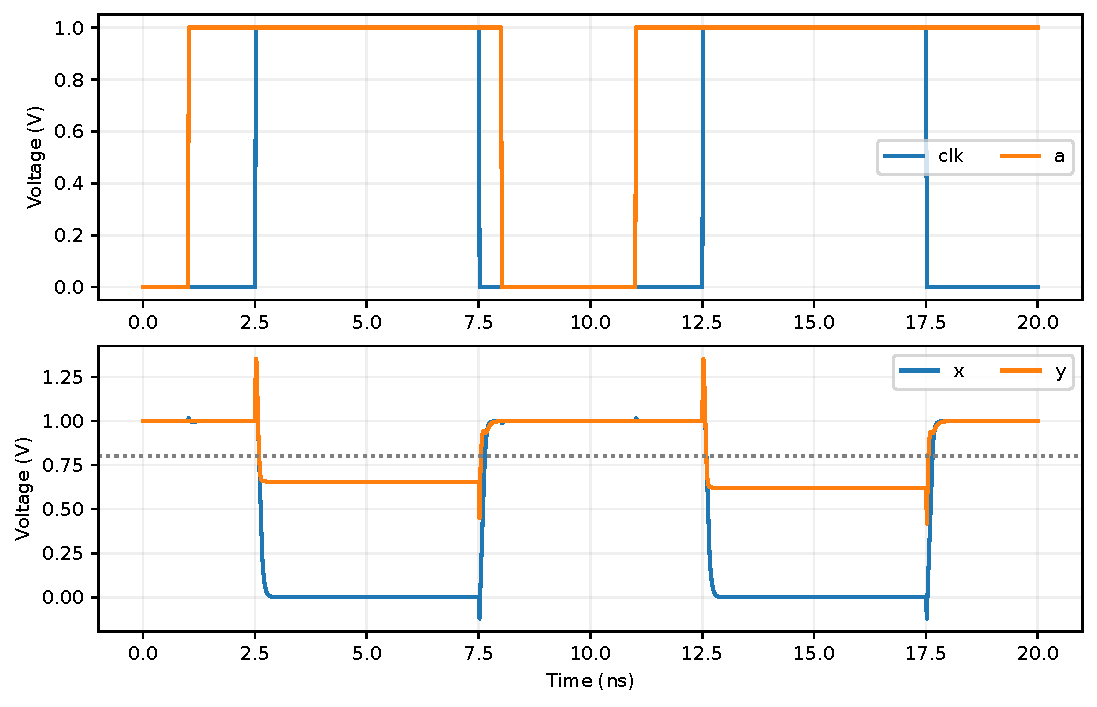
\includegraphics[width=.93\linewidth]{figures/unsafe_cascade.pdf}
\caption{Charge loss in the direct cascade; dotted line is the 0.8 V diagnostic threshold.}
\end{figure}

\section{Step 2: equal-noise comparison}

A is fixed at zero, so both outputs should remain low. During evaluation, aggressor Q falls from 1 to 0 V at 4 ns and couples through equal capacitances into each first dynamic node. The handout condition is 10 fF. A static inverter in N-domino rejects small disturbances, whereas N-P stages directly control opposite-type devices and can regenerate smaller floating-node shifts.

\begin{center}\small
\begin{tabular}{lrr}
\toprule
C (fF) & N peak (V) & N-P peak (V) \\
\midrule
0.001 & -0.000011 & -0.096783 \\
2 & 0.000056 & -0.096796 \\
5 & 0.000141 & -0.096797 \\
10 & 0.000249 & 0.999901 \\
15 & 0.000443 & 1.000282 \\
20 & 1.006744 & 1.001090 \\
30 & 1.010412 & 1.001674 \\
\bottomrule
\end{tabular}
\end{center}

\begin{figure}[htbp]\centering
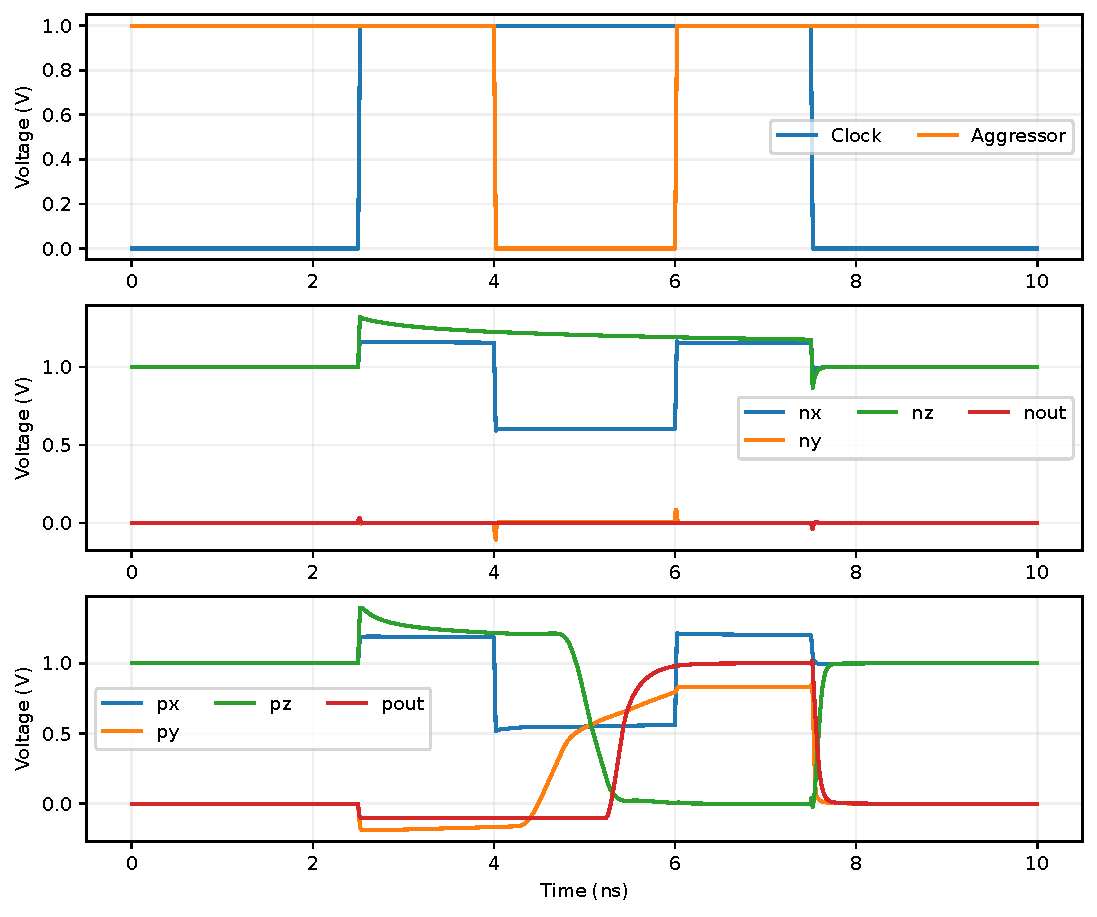
\includegraphics[width=.93\linewidth]{figures/equal_noise.pdf}
\caption{Equal 10 fF disturbances and the internal nodes of each chain.}
\end{figure}

At 10 fF the N-domino peak is only 0.000249 V, while the N-P output reaches approximately 1 V and holds an erroneous high. The distinction persists at 15 fF, whereas both fail at 20/30 fF. The near-zero 0.001 fF control shows N-P clock feedthrough near -0.097 V, which is not clipped to ideal zero. These tests support better N-domino immunity under the stated conditions, not under every sizing, edge, load, or noise waveform.

\section{Q1: speed and discussion}

A separate input transition at 4 ns during evaluation compares data-path speed without confusing precharge timing with propagation delay. Using 0.5 V input/output crossings, N-domino delay is 367.720 ps and N-P delay is 657.328 ps. N-domino is faster in this implementation. Eliminating static inverters does not by itself guarantee a faster N-P chain: PMOS stack drive, node loading, and device sizes also contribute.

\begin{figure}[htbp]\centering
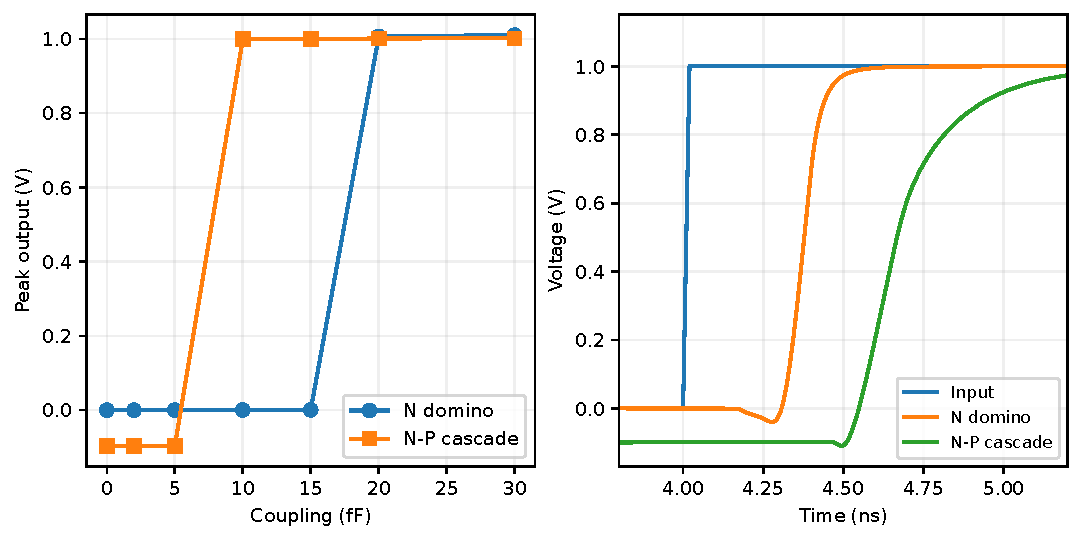
\includegraphics[width=.93\linewidth]{figures/sweep_and_speed.pdf}
\caption{Left: coupling sweep. Right: data-path speed test without coupling capacitors.}
\end{figure}

A precharged output must not enable the next evaluation network. Same-type stages therefore need an intervening inverter, while opposite types can connect directly, with analog noise tolerance still requiring evaluation. These are finite circuit simulations, not PVT, post-layout, or complete noise signoff.
